\subsection{bpmnr/nr\_\-checks.c File Reference}
\label{nr__checks_8c}\index{bpmnr/nr\_\-checks.c@{bpmnr/nr\_\-checks.c}}


\subsubsection{Detailed Description}


Definition in file {\bf nr\_\-checks.c}.

{\tt \#include $<$bpm/bpm\_\-messages.h$>$}\par
{\tt \#include $<$bpm/bpm\_\-nr.h$>$}\par


Include dependency graph for nr\_\-checks.c:\nopagebreak
\begin{figure}[H]
\begin{center}
\leavevmode
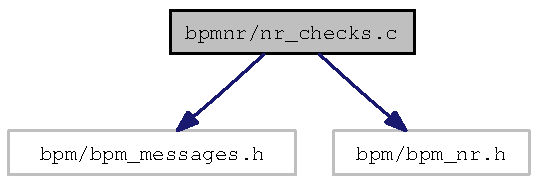
\includegraphics[width=147pt]{nr__checks_8c__incl}
\end{center}
\end{figure}
\subsubsection*{Functions}
\begin{CompactItemize}
\item 
int {\bf nr\_\-is\_\-int} (double x)
\item 
int {\bf nr\_\-is\_\-pow2} (unsigned long n)
\end{CompactItemize}


\subsubsection{Function Documentation}
\index{nr\_\-checks.c@{nr\_\-checks.c}!nr\_\-is\_\-int@{nr\_\-is\_\-int}}
\index{nr\_\-is\_\-int@{nr\_\-is\_\-int}!nr_checks.c@{nr\_\-checks.c}}
\paragraph[nr\_\-is\_\-int]{\setlength{\rightskip}{0pt plus 5cm}int nr\_\-is\_\-int (double {\em x})}\hfill\label{nr__checks_8c_0f1f21216d96e661d4ba6b91e91538ed}


Checks whether the given double is an integer value, handy for doing domain checking to prevent e.g. the function nr\_\-gammln print out \char`\"{}nan\char`\"{} or \char`\"{}inf\char`\"{} values...

For double precision, this check is accurate to 1.0E-323 ... should be enough ;-)

\begin{Desc}
\item[Parameters:]
\begin{description}
\item[{\em x}]floating point argument\end{description}
\end{Desc}
\begin{Desc}
\item[Returns:]TRUE if argument is indeed an integer value, FALSE if not \end{Desc}


Definition at line 21 of file nr\_\-checks.c.

Referenced by nr\_\-gammln().